\documentclass[11pt,a4paper]{article}
\usepackage[margin=25mm]{geometry}
\usepackage{fontspec}
\setmainfont{TeX Gyre Pagella}
\setsansfont{TeX Gyre Heros}
\usepackage[french]{babel}
\usepackage{amsmath,amssymb,booktabs,tabularx,graphicx,float,placeins}
\usepackage{unicode-math}
\setmathfont{TeX Gyre Pagella Math}
\usepackage[authoryear,round]{natbib}
\usepackage{xcolor}
\usepackage{hyperref}
\usepackage{xurl}
\hypersetup{colorlinks=true,linkcolor=blue!45!black,citecolor=blue!45!black,urlcolor=blue!45!black,pdfauthor={Kun Huang}}
\usepackage{caption}
\captionsetup{font=small,labelfont=bf}
\setlength{\parskip}{4pt}
\setlength{\parindent}{14pt}
\setlength{\emergencystretch}{2em}
\renewcommand{\arraystretch}{1.15}
\newcommand{\notes}[1]{\par\vspace{3pt}{\footnotesize\noindent\textit{Note :} #1\par}}
\newcommand{\source}[2]{\href{#1}{#2}}
\newcommand{\BorderCoef}{0,146}
\newcommand{\BorderLo}{0,051}
\newcommand{\BorderHi}{0,241}
\newcommand{\BorderSE}{0,048}
\newcommand{\BroadCoef}{-0,007}
\newcommand{\BroadLo}{-0,065}
\newcommand{\BroadHi}{0,052}
\newcommand{\MatchedCoef}{-0,017}
\newcommand{\MatchedLo}{-0,100}
\newcommand{\MatchedHi}{0,066}
\newcommand{\BorderPairs}{774}
\newcommand{\NewN}{2\,117}
\newcommand{\ControlN}{14\,361}
\newcommand{\MatchedPairs}{1\,908}
\newcommand{\PanelN}{3\,068\,820}
\newcommand{\CommuneN}{34\,098}
\newcommand{\BirthN}{11\,285\,045}
\newcommand{\ULBirthN}{6\,953\,847}
\newcommand{\ShortPreP}{0,489}
\newcommand{\SeasonPreP}{0,000157}
\newcommand{\AnnualPreP}{0,238}
\newcommand{\PPMLRatio}{1,056}
\newcommand{\MapFRRN}{17\,622}
\newcommand{\PPMLPairs}{757}
\newcommand{\PPMLExcluded}{17}
\newcommand{\WildP}{0,0077}
\newcommand{\FRRInitialN}{17\,717}
\newcommand{\FRRInitialPartialN}{20}
\newcommand{\OldZRRFullN}{17\,694}
\newcommand{\OldZRRPartialN}{36}
\newcommand{\FRRAdditionsAprN}{117}
\newcommand{\FRRCoreJulyN}{17\,789}
\newcommand{\FRRCorePartialJulyN}{20}
\newcommand{\FRRBenefJulyN}{2\,145}
\newcommand{\FRRBenefPartialJulyN}{11}
\newcommand{\FRRPlusJulyN}{4\,456}
\newcommand{\StableNeverN}{14\,611}
\newcommand{\StableLaterCoreExcludedN}{116}
\newcommand{\BorderCommuneN}{1\,548}
\newcommand{\EPCIComponentsN}{128}
\newcommand{\EDComponentsN}{46}
\newcommand{\EDBComponentsN}{36}
\newcommand{\EDBMaxPairsN}{191}
\newcommand{\HQBirthN}{10\,175\,417}
\newcommand{\NonHQBirthN}{1\,101\,326}
\newcommand{\UnknownHQN}{8\,302}
\newcommand{\UnknownAgeN}{29\,742}
\newcommand{\AgeFlaggedN}{24}
\newcommand{\AssignmentMetroN}{34\,816}
\newcommand{\AssignmentListedN}{17\,672}
\newcommand{\AssignmentMandatoryN}{14\,316}
\newcommand{\AssignmentResidualN}{3\,356}
\newcommand{\AssignmentUnlistedN}{17\,144}
\newcommand{\AssignmentBOnlyN}{3\,013}
\newcommand{\AssignmentDOnlyN}{304}
\newcommand{\AssignmentBothN}{39}
\newcommand{\AssignmentBOnlyBVN}{314}
\newcommand{\EPCIIncomeCut}{21570}
\newcommand{\EPCIDensityCut}{63,57}
\newcommand{\BVIncomeCut}{21600}
\newcommand{\BVDensityCut}{70,84}
\newcommand{\IncomeRDEligibleN}{6}
\newcommand{\DensityRDEligibleN}{1}
\newcommand{\AssignmentFieldChecksN}{1\,044\,480}
\newcommand{\BVRDCoef}{0,444}
\newcommand{\BVRDLo}{-0,024}
\newcommand{\BVRDHi}{0,912}
\newcommand{\BVRDEligibleN}{119}
\newcommand{\BVRDControlN}{79}
\newcommand{\BVRDGroupN}{33}
\newcommand{\BVRDFullGroupN}{10}
\newcommand{\BVRDCoverageJump}{-44,4}
\newcommand{\BVRDCoverageLo}{-71,9}
\newcommand{\BVRDCoverageHi}{-16,9}
\newcommand{\BVRDCoverageHolmP}{0,072}
\newcommand{\BVRDOldShareJump}{30,7}
\newcommand{\BVRDFullMaxShare}{79,3}
\newcommand{\BVRDCovariateN}{63}
\newcommand{\BVRDTestableCovN}{46}
\newcommand{\BVRDPreN}{53}
\newcommand{\BVRDClusterRank}{32}
\newcommand{\BVRDFullRank}{9}


\hypersetup{pdftitle={Reconstruire l'éligibilité à France ruralités revitalisation : données publiques, immatriculations et limites de l'évaluation de 2024}}
\title{Reconstruire l’éligibilité à France ruralités revitalisation :\\données publiques, immatriculations et limites de l’évaluation de 2024}
\author{Kun Huang\thanks{Economics and Management School, Wuhan University, Wuhan, China. Courriel : \href{mailto:huangkun123huang@163.com}{huangkun123huang@163.com}. La déclaration finale décrit l’assistance substantielle de Codex et la portée des vérifications internes.}}
\date{4 octobre 2026 — document de travail}
\begin{document}
\maketitle
\begin{abstract}
Cet article reconstitue l’exposition à la réforme France ruralités revitalisation (FRR) et examine ce que les données publiques permettent d’évaluer. Les données de 2020 de l’Institut national de la statistique et des études économiques (INSEE), dans la géographie de 2023, permettent de reproduire les seuils nationaux utilisés pour le classement initial. Parmi les \AssignmentListedN{} communes métropolitaines initialement classées, \AssignmentMandatoryN{} satisfont au moins une voie de classement obligatoire vérifiée ; les \AssignmentResidualN{} autres relèvent de voies possibles à l’échelle des bassins de vie ou des zones de montagne. L’union des voies ainsi reconstruites reproduit exactement la liste, sans révéler les décisions préfectorales individuelles ni la population résidant dans les seules parties classées en zone de montagne. La transition des zones de revitalisation rurale (ZRR) vers FRR est ensuite reliée à un panel mensuel SIRENE de janvier 2019 à juin 2026, fondé sur les localisations et les états administratifs historiques. Pour juillet–décembre 2024, les contrastes larges et appariés sont proches de zéro, tandis que le contraste estimé dans \BorderPairs{} paires frontalières s’élève à \BorderCoef{} immatriculation mensuelle par mille habitants (intervalle à 95 \% : [\BorderLo{} ; \BorderHi{}]). Les écarts observés sur l’ensemble de la période préalable ne permettent toutefois pas de justifier une interprétation causale de ces comparaisons. Après exclusion des voies alternatives d’éligibilité, le nombre d’intercommunalités comparables de part et d’autre des seuils est insuffisant pour une estimation en discontinuité. L’analyse au seuil de revenu des bassins porte sur davantage d’unités comparables, mais présente des écarts de couverture et des discontinuités préalables qui empêchent également une interprétation causale. L’étude fournit une reconstruction reproductible de l’exposition, des mesures administratives et des diagnostics sur les limites de l’évaluation initiale. Elle n’établit ni création nette nationale, ni hausse de l’emploi, ni inefficacité du dispositif.
\end{abstract}
\noindent\textbf{Mots-clés :} fiscalité territoriale ; France ruralités revitalisation ; SIRENE ; immatriculations ; frontières communales ; identification.\\
\textbf{Codes JEL :} H25, H71, R38, L26.

\section{Introduction}
Les dispositifs territoriaux de soutien aux entreprises cherchent à modifier les choix de localisation et à soutenir l’activité dans les espaces où les conditions économiques sont défavorables. Leur évaluation doit distinguer l’attraction locale d’établissements de la création d’activité à une échelle plus large. Elle doit aussi distinguer l’éligibilité géographique d’une entreprise du bénéfice effectif d’une exonération.

Le nouveau zonage France ruralités revitalisation remplace les zones de revitalisation rurale (ZRR) à compter du 1er juillet 2024. Cette transition ne constitue pas une expérience où toutes les communes classées commencent simultanément à bénéficier d’un soutien. Beaucoup étaient déjà classées en ZRR ou conservaient les effets de ce classement. D’autres continuent à bénéficier d’avantages sans figurer dans la liste initiale FRR. Une comparaison de l’ensemble des communes FRR à l’ensemble des communes non FRR mélange donc des situations institutionnelles différentes.

La première question porte sur la mesure de l’exposition : peut-on relier la décision de 2024 à ses critères d’origine, sans confondre classement, maintien d’anciens droits et bénéfice fiscal effectivement reçu ? La seconde concerne l’information économique accessible au public : quelles évolutions administratives peut-on décrire, et quelles hypothèses supplémentaires seraient nécessaires pour les attribuer à FRR ? Ces questions commandent l’ordre de l’analyse. Un classement correctement téléchargé n’est ni une mesure de l’exonération reçue, ni un mécanisme d’assignation déjà identifié.

L’étude utilise exclusivement des données gratuites d’institutions publiques françaises. Elle retrouve les données de 2020 et les périmètres de 2023 utilisés pour le classement initial, reproduit les seuils nationaux et confronte les voies juridiques à l’ensemble des communes métropolitaines. Elle reconstruit ensuite les séries d’immatriculations dans les communes qui ne relevaient auparavant ni du zonage ZRR ni du maintien de ses effets. Le registre SIRENE permet de séparer unités légales et établissements, d’exploiter les historiques administratifs et de repérer certaines continuités économiques enregistrées. Il ne mesure ni les profits, ni les exonérations perçues, ni la production. Le champ des observations est ainsi plus étroit que celui de la création d’activité économique.

L’analyse privilégie les voisins situés de part et d’autre d’une frontière du zonage. Cette restriction vise à rendre les conditions locales plus comparables, sans rendre le classement aléatoire. La comparaison large et l’appariement sur des caractéristiques préalables sont conservés pour montrer la dépendance des résultats au choix du contrefactuel. Les périodes d’annonce et les renforcements ultérieurs sont séparés de la fenêtre initiale d’exposition.

La contribution repose sur une reconstruction vérifiable de l’exposition et un diagnostic des limites de son évaluation. À l’échelle métropolitaine, la correspondance entre la liste et l’union des voies de classement compatibles avec les critères numériques, la séparation des voies obligatoires et incertaines, et le petit nombre d’établissements publics de coopération intercommunale (EPCI) comparables au voisinage des seuils après exclusion des voies alternatives apportent des informations distinctes du nombre de communes publié dans l’arrêté. Le panel historique explicite les différences entre immatriculation, siège, unité légale, continuité enregistrée et maintien administratif. Enfin, les comparaisons locales et larges montrent pourquoi un contraste frontalier positif ne suffit pas à conclure à une réponse causale. Les diagnostics pouvant invalider cette interprétation sont des résultats de l’étude. Le journal des décisions méthodologiques distingue les choix faits avant les premières estimations de la recherche de seuils conduite après leur lecture ; il ne constitue pas un pré-enregistrement externe.

\section{Travaux antérieurs}
Les évaluations de ZRR constituent le point de départ pertinent. L’étude de \citet{ref0} examine les effets des exonérations sur les établissements et l’emploi par une approche en discontinuité. \citet{ref1} exploitent les discontinuités d’un ancien mécanisme de classement rural et rapportent une absence d’effet détectable sur plusieurs indicateurs. Ces travaux portent sur des versions antérieures de la politique. Leurs règles de classement, leurs périodes et leurs données ne peuvent être transférées directement à la réforme de 2024.

Les études françaises des zones franches urbaines montrent pourquoi la localisation des créations importe. \citet{ref2} examinent notamment les externalités sur les zones voisines ; \citet{ref4} analysent les décisions de localisation des établissements. \citet{ref3} distinguent l’attraction initiale et la persistance des résultats. \citet{ref5} montrent que l’intégration géographique et l’accessibilité peuvent modifier la réponse au soutien territorial. Ces politiques urbaines ne sont pas des analogues institutionnels parfaits de FRR ; elles motivent une vérification des déplacements et de la durabilité plutôt qu’un effet attendu imposé à l’avance.

L’incidence et le bien-être nécessitent des résultats plus riches que les entrées au registre, comme l’illustre l’étude de \citet{ref6}. Les effets fixes paire–période s’inscrivent dans la tradition des comparaisons de territoires contigus \citep{ref9}. Cette méthode exige toutefois de gérer les unités répétées et leur dépendance. Les travaux de \citet{ref7,ref8} montrent qu’un témoin voisin peut être affecté par le traitement ; l’estimation soustrait alors sa réponse indirecte. Enfin, \citet{ref10} proposent une analyse des écarts admissibles aux tendances parallèles. Le non-rejet d’un test préalable ne constitue pas une validation de cette hypothèse. Le présent travail ne prétend pas appliquer leur procédure de bornes ni reproduire un estimateur utilisant des adresses d’établissements géocodées.

\section{Institution et reconstruction du traitement}
\subsection{La réforme initiale et les annonces}
Le plan France Ruralités est annoncé le 15 juin 2023. L’article 73 de la loi de finances pour 2024 crée le dispositif ; l’arrêté du 19 juin 2024 est publié le 20 juin et prend effet le 1er juillet. Son annexe, fondée sur le code officiel géographique (COG) 2023, contient \FRRInitialN{} codes distincts, dont \FRRInitialPartialN{} communes de La Réunion partiellement zonées. Ces derniers codes ne représentent pas des communes entièrement éligibles. Les textes originaux, et non leurs seules versions consolidées en 2026, sont utilisés pour documenter le régime de 2024.\footnote{\source{https://www.legifrance.gouv.fr/jorf/article_jo/JORFARTI000048727426}{Loi de finances pour 2024, article 73} ; \source{https://www.legifrance.gouv.fr/jorf/id/JORFTEXT000049746820}{arrêté initial du 19 juin 2024}. L’annonce générale est documentée par le ministère : \source{https://www.ecologie.gouv.fr/presse/france-ruralites-plan-ambitieux-davantage-dequite-territoriale}{France Ruralités, 15 juin 2023}.}

Le canal de droit commun combine une population communale inférieure à 30\,000 habitants avec des critères de densité et de revenu de l’EPCI comparés aux médianes métropolitaines. Le texte comporte aussi des voies départementales, de montagne et de bassin de vie. Pour le classement initial, la loi retient les données disponibles au 1er juillet 2023 et le périmètre des EPCI arrêté au 1er janvier 2023 ; ces dates ne signifient pas que toutes les variables économiques sont observées en 2023. Le fichier de classement indique le résultat de ces voies, mais pas la voie effectivement déterminante pour chaque commune.

\subsection{Retrouver les variables et les voies de la première décision}
Le compte rendu parlementaire contemporain confirme l’emploi du recensement et des fichiers Filosofi, tous deux de 2020. Les tables de revenus diffusées le 24 avril 2023 et la série historique de population diffusée le 27 juin 2023 sont disponibles avant la date légale. La densité est le rapport entre la somme des populations municipales et celle des superficies dans chaque périmètre officiel. Le plafond communal est appliqué à la population municipale de 2020. Le revenu est la médiane du niveau de vie, soit le revenu disponible du ménage par unité de consommation. Les médianes publiées par l’INSEE à l’échelle des EPCI, des bassins de vie et des départements sont utilisées séparément : une moyenne des médianes communales ne reconstituerait pas la médiane du niveau de vie de ces territoires.\footnote{\source{https://www.senat.fr/cra/s20231126/s20231126.pdf}{Sénat, séance du 26 novembre 2023}, p. 63 dans la pagination imprimée ; \source{https://www.insee.fr/fr/statistiques/6692392}{Filosofi 2020} ; \source{https://www.insee.fr/fr/statistiques/7632565}{séries historiques du recensement 2020}. Les archives exactes et leurs empreintes figurent dans le manifeste.}

Les seuils du tableau~\ref{tab:thresholds} correspondent aux valeurs officielles décrivant les règles de la loi de finances pour 2024. Les densités affichées sont arrondies ; les tests emploient les médianes recalculées avant arrondi. La voie de droit commun A requiert densité et revenu EPCI inférieurs ou égaux aux médianes. La voie départementale C retient une densité strictement inférieure à 35 et un niveau de vie médian inférieur ou égal à la médiane des niveaux de vie médians par département ; treize départements satisfont cette intersection. La voie de montagne D conserve le seuil de densité EPCI, relève celui de revenu au troisième quartile et exige au moins la moitié de la population dans les zones définies par l’article 3 de la loi Montagne de 1985. La voie de bassin B requiert le respect des deux seuils de bassin, une proposition du préfet de région motivée par l’intérêt général et un classement par arrêté interministériel. La limite de population s’applique à la commune à classer : une grande ville membre d’un bassin ne rend pas tous les autres membres inéligibles.\footnote{\source{https://www.legifrance.gouv.fr/codes/article_lc/LEGIARTI000049130324/2024-07-01/}{CGI 44 quindecies A, version du 1er juillet 2024}, II et IV ; \source{https://www.assemblee-nationale.fr/dyn/17/rapports/cion-dvp/l17b0486-tviii_rapport-avis.pdf}{Assemblée nationale, avis n° 486-VIII, 25 octobre 2024}, p. 18.}

\begin{table}[htbp]\centering\small\caption{Seuils reproduits pour le classement initial de 2024}\label{tab:thresholds}\begin{tabularx}{\linewidth}{Xrrr}
\toprule
Périmètre & Unités & Densité & Niveau de vie \\
\midrule
EPCI de droit commun & 1\,232 & 63,57 & 21570 \\
EPCI, voie montagne & 1\,232 & 63,57 & 22822,5 \\
Bassins de vie & 1\,681 & 70,84 & 21600 \\
Départements & 96 & strictement < 35 & 21665 \\
\bottomrule
\end{tabularx}
\notes{Population et niveau de vie de 2020, géographie au 1er janvier 2023. Densité en habitants/km\textsuperscript{2}, niveau de vie en euros par unité de consommation. Les unités sont les périmètres métropolitains de référence, pas le nombre d’unités éligibles. Hormis la condition départementale strictement <35, les seuils sont inclusifs. Les autres conditions légales ne sont pas contenues dans ces seules colonnes.}\end{table}

La reconstruction porte sur \AssignmentMetroN{} communes métropolitaines du COG 2023, dont \AssignmentListedN{} figurent dans l’arrêté initial. Les quatre communes sans EPCI emploient leurs propres indicateurs dans la voie A ; le code « sans objet » ne correspond pas à un EPCI commun à ces quatre îles. Un revenu communal non diffusé reste inconnu. Il n’est pas imputé ; une autre condition nécessaire connue comme non satisfaite peut cependant exclure la voie sans connaître ce revenu.

Le fichier officiel de montagne, mis à jour le 23 mars 2022 en COG 2022, identifie les communes concernées, y compris certaines parties de communes, et les fusions historiques. Les mouvements entre les périmètres 2022 et 2023 sont vérifiés séparément, y compris lorsque le code reste identique. Ce fichier ne fournit pas la population résidant dans les seules parties classées. La population totale des communes concernées, ou dont la correspondance est incertaine, définit donc un \emph{majorant} de la part de population de montagne. Ce majorant reste conditionnel à la couverture de cette archive ; les mouvements administratifs ne reconstituent ni la population infracommunale ni d’éventuelles modifications du zonage juridique absentes du fichier. Les critères numériques de la voie B définissent une qualification possible, sans que les propositions préfectorales soient observées. Ces limites sont maintenues dans les indicateurs : « possible » n’est jamais remplacé par « effectivement accordé par cette voie ».\footnote{\source{https://www.data.gouv.fr/datasets/communes-de-la-loi-montagne-au-code-officiel-geographique-cog-2020-2022}{Communes de la loi Montagne, ministère chargé de la cohésion des territoires}. Ce périmètre légal ne se confond pas avec celui des massifs.}

\begin{table}[htbp]\centering\small\caption{Confrontation des voies reconstruites à la liste métropolitaine initiale}\label{tab:paths}\begin{tabularx}{\linewidth}{Xrr}
\toprule
Relation aux critères reconstruits & Dans la liste & Hors liste \\
\midrule
Au moins une voie obligatoire A ou C & 14\,316 & 0 \\
Bassin seul parmi les voies restantes & 3\,013 & 0 \\
Montagne possible seule & 304 & 0 \\
Bassin et montagne possibles & 39 & 0 \\
Aucune voie possible reconstruite & 0 & 17\,144 \\
Total & 17\,672 & 17\,144 \\
\bottomrule
\end{tabularx}
\notes{Les voies obligatoires vérifiées regroupent A, y compris les communes sans EPCI, et C. Les lignes suivantes sont exclusives parmi les communes sans voie obligatoire. B désigne les conditions numériques de bassin ; D une possibilité au regard du majorant de population de montagne. La correspondance de l’union avec la liste ne révèle pas la voie administrative effectivement utilisée.}\end{table}

Toutes les \AssignmentMandatoryN{} communes satisfaisant une voie obligatoire vérifiée figurent dans la liste. Les \AssignmentResidualN{} autres communes classées disposent d’une possibilité B ou D. Parmi elles, \AssignmentBOnlyN{} n’ont que B comme voie restante, \AssignmentDOnlyN{} que D au regard du majorant, et \AssignmentBothN{} les deux. Le premier sous-ensemble concerne \AssignmentBOnlyBVN{} bassins ; il exige une décision complémentaire dans le cadre des voies reconstruites, sans constituer une liste officielle de propositions reçues ou approuvées. Aucune commune non classée ne satisfait une voie possible ainsi reconstruite. Cette égalité des ensembles est une vérification nationale de cohérence, pas une observation des raisons individuelles ni une preuve d’exogénéité de la décision.
\FloatBarrier

\subsection{Un ensemble d’avantages sous conditions}
Dans le dispositif FRR socle, l’exonération nationale d’impôt sur les bénéfices concerne les entreprises créées ou reprises du 1er juillet 2024 au 31 décembre 2029, remplissant notamment des conditions relatives à l’activité, à l’implantation, au régime réel d’imposition et à un effectif de moins de onze salariés. Elle couvre la période allant jusqu’au terme du cinquante-neuvième mois suivant celui de la création ou de la reprise, puis des exonérations partielles de 75, 50 et 25 \% sur trois périodes de douze mois. Il ne suffit donc pas qu’une entreprise existante ouvre un établissement dans une commune FRR pour remplir toutes ces conditions.

La cotisation foncière des entreprises (CFE) et la taxe foncière sur les propriétés bâties (TFPB) requièrent des délibérations locales distinctes, pour la part de chaque collectivité concernée. Pour un établissement créé par une entreprise bénéficiant de l’exonération de bénéfices, la CFE peut être exonérée pendant cinq années à compter de l’année suivant la création, puis sa base peut être réduite de 75, 50 et 25 \% durant les trois années suivantes. La TFPB concerne un immeuble rattaché à un établissement remplissant les conditions de la CFE ; l’exonération suit les mêmes proportions et durée, à compter du 1er janvier suivant le rattachement. Les demandes et déclarations requises doivent aussi être effectuées. La fenêtre exceptionnelle de délibération de 2024 se termine le 18 septembre inclus pour permettre une application dès les impositions de 2025. Ce millésime correspond notamment aux créations et rattachements éligibles de 2024, sous réserve des autres conditions. Aucun inventaire national officiel complet des décisions effectivement adoptées n’a été vérifié pour cette étude ; le classement ne mesure donc pas le bénéfice effectif de ces exonérations locales.\footnote{Article 73, CGI 44 quindecies A, 1466 G et 1383 K ; \source{https://www.collectivites-locales.gouv.fr/files/files/3.\%20Animer\%20les\%20territoires/5.\%20La\%20coh\%C3\%A9sion\%20territoriale\%20et\%20l'am\%C3\%A9nagement\%20du\%20territoire/FAQ\%20FRR_MAJ\%20juillet2025.pdf}{FAQ officielle DGCL, juillet 2025}, notamment p. 16.}

Le régime national exonère, pour les embauches éligibles, les cotisations patronales d’assurances sociales et d’allocations familiales pendant douze mois. La rédaction historique exclut une embauche portant l’effectif total de l’entreprise à au moins cinquante salariés ; l’exonération est pleine jusqu’à 1,5 SMIC, décroît ensuite et devient nulle à partir de 2,4 SMIC. L’employeur ne doit pas avoir procédé à un licenciement économique dans les douze mois précédents. Le contrat doit être un CDI ou un CDD admissible d’au moins douze mois ; la déclaration historique doit être transmise dans les trente jours. L’indicateur employeur de SIRENE ne permet pas de vérifier ces conditions ni de mesurer la réduction de cotisations effectivement obtenue.\footnote{\source{https://www.legifrance.gouv.fr/codes/article_lc/LEGIARTI000048846858/2025-02-28}{CSS L241-19, version historique 2024–2025}. Aucun montant monétaire de SMIC de 2026 n’est appliqué rétrospectivement.}

Le traitement empirique est le classement territorial. Même si les hypothèses d’identification étaient satisfaites, l’estimation aurait l’interprétation d’un effet en intention de traiter lié à ce classement, et non l’effet de recevoir un montant particulier de réduction fiscale. FRR s’inscrit également dans une politique rurale comportant des dispositifs non fiscaux.

\subsection{ZRR antérieures, maintien et modifications ultérieures}
La situation territoriale avant réforme repose sur l’arrêté du 16 mars 2017 modifié le 22 février 2018, ainsi que sur les dispositifs de maintien des effets pour les communes sorties du classement en 2017. L’article 73, XVI et XVII, de la loi de finances pour 2024 prolonge ces dispositifs de maintien jusqu’au 30 juin 2024. Le fichier officiel ANCT en COG 2021 convertit cette géographie et distingue les situations de classement et de maintien. La stabilité du code et du territoire est contrôlée ; les communes dont la correspondance n’est pas sûre sont exclues. L’arrêté ZRR du 19 juin 2024 entre en vigueur le 1er juillet et ne fournit pas une nouvelle liste à utiliser au 30 juin.\footnote{\source{https://www.legifrance.gouv.fr/loda/id/JORFTEXT000034298773/2018-04-01}{Liste historique ZRR} ; \source{https://static.data.gouv.fr/resources/zones-de-revitalisation-rurale-zrr/20210907-124104/diffusion-zonages-zrr-cog2021.xls}{conversion officielle ANCT COG 2021} ; \source{https://www.legifrance.gouv.fr/jorf/id/JORFTEXT000049746830}{arrêté ZRR du 19 juin 2024}.}

La loi de finances pour 2025 ajoute des voies de classement et accorde les effets FRR aux communes auparavant classées en ZRR ou bénéficiant de ses effets, qui ne sont pas reclassées en FRR. Ce maintien, prévu à l’article 99, IV, s’applique rétroactivement au 1er juillet 2024 en vertu du VII-A ; les autres modifications doivent être suivies selon leurs propres clauses d’entrée en vigueur. L’arrêté du 14 avril 2025 publie les classements complémentaires et les communes bénéficiaires. Le décret de mise en œuvre et l’arrêté de classement FRR+ sont publiés le 10 juillet 2025, avec effet juridique au 1er janvier 2025. La loi de finances pour 2026 prolonge jusqu’en 2029 le terme des effets pour les communes bénéficiaires concernées, sans leur conférer le statut FRR+. Ces communes ne sont jamais utilisées comme témoins non bénéficiaires.\footnote{\source{https://www.legifrance.gouv.fr/jorf/article_jo/JORFARTI000051168986}{Loi de finances pour 2025, article 99} ; \source{https://www.legifrance.gouv.fr/jorf/id/JORFTEXT000051469445}{arrêté du 14 avril 2025} ; \source{https://www.legifrance.gouv.fr/jorf/id/JORFTEXT000051871894}{décret FRR+} et \source{https://www.legifrance.gouv.fr/jorf/id/JORFTEXT000051871914}{arrêté FRR+} ; \source{https://www.legifrance.gouv.fr/jorf/article_jo/JORFARTI000053508415}{loi de finances pour 2026, article 48}.}

La fenêtre principale s’arrête donc en décembre 2024. La période juillet 2024–juin 2025 ne serait pas une année d’exposition au seul dispositif FRR socle pour les communes devenues FRR+. L’annonce de 2023 et la loi de décembre 2023 motivent l’exclusion de juin 2023–juin 2024 de la moyenne de référence, sans supposer que toute anticipation est ainsi éliminée.

\begin{table}[htbp]\centering\small\caption{Transitions du zonage : univers courant et échantillon stable}\label{tab:transitions}\begin{tabularx}{\linewidth}{Xrr}
\toprule
Transition & Codes courants DGCL & Métropole stable \\
\midrule
Non-ZRR → FRR initiale & 2\,161 & 2\,117 \\
ZRR → FRR initiale & 15\,478 & 15\,164 \\
ZRR → maintien des effets & 2\,133 & 2\,090 \\
Non-ZRR → non-FRR & 14\,935 & 14\,611 \\
Partiel ou non résolu & 168 & 116 \\
\bottomrule
\end{tabularx}
\notes{L’univers courant est celui des codes DGCL de juillet 2025, pas des codes historiques de l’arrêté. « ZRR » comprend le maintien des effets. Le filtre stable exclut les mouvements COG autres que les changements de nom depuis 2017, les statuts partiels et les changements d’EPCI entre 2023 et 2024. Dans la colonne stable, la dernière ligne comprend \StableLaterCoreExcludedN{} codes de classement ultérieur, et aucun statut partiel ; ces codes n’entrent dans aucune des trois comparaisons.}\end{table}
\begin{figure}[htbp]\centering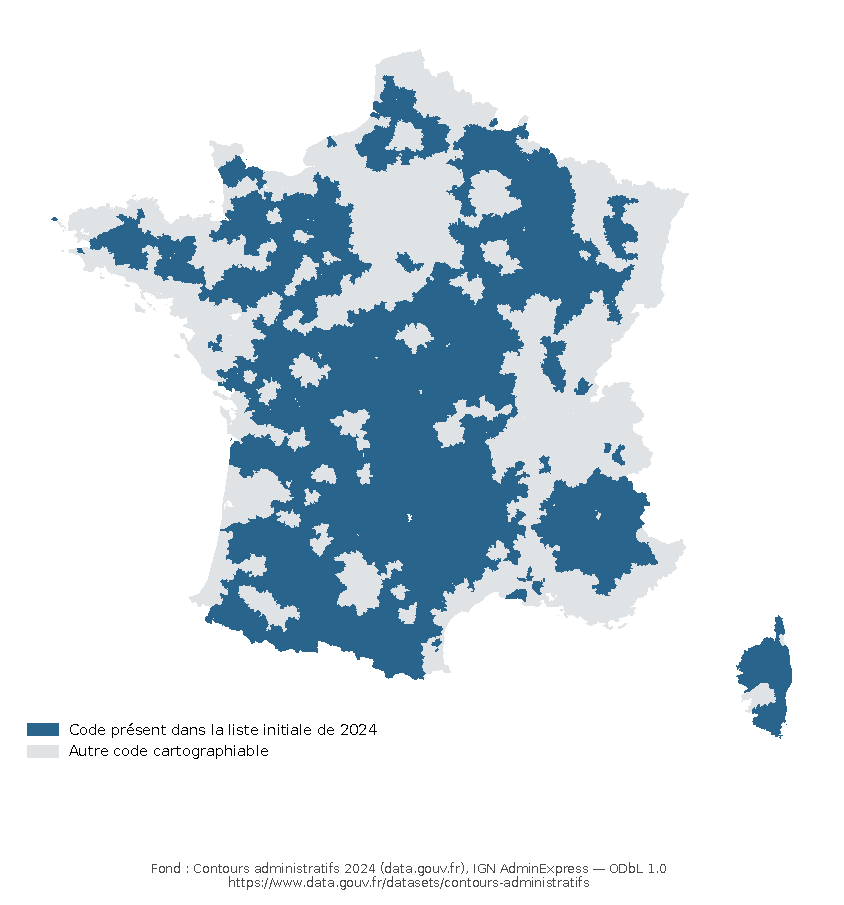
\includegraphics[width=.70\linewidth]{../results/figures/frr_map.pdf}\caption{Liste initiale FRR de 2024 dans les contours métropolitains directement appariables}\label{fig:map}\notes{\MapFRRN{} codes initiaux sont cartographiables dans l’univers courant retenu. Cette représentation exclut l’outre-mer et ne reconstitue pas les territoires fusionnés ; elle n’est pas la carte exhaustive des codes COG 2023. Contours administratifs 2024 diffusés par data.gouv.fr, issus d’IGN AdminExpress, sous \source{https://opendatacommons.org/licenses/odbl/1-0/}{ODbL 1.0} ; simplification pour l’affichage seulement.}\end{figure}
\begin{figure}[htbp]\centering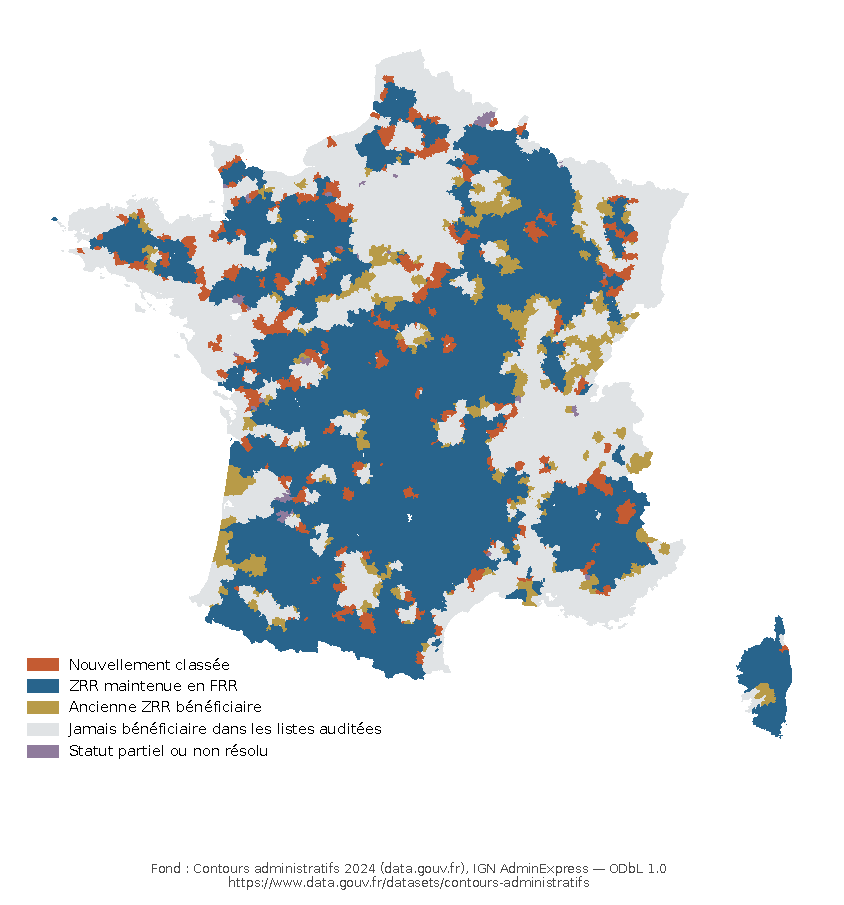
\includegraphics[width=.70\linewidth]{../results/figures/transition_map.pdf}\caption{Transition ZRR–FRR dans la même couverture cartographique}\label{fig:transition}\notes{Sources : ANCT, Légifrance, DGCL, INSEE ; Contours administratifs 2024, data.gouv.fr/IGN AdminExpress, \source{https://opendatacommons.org/licenses/odbl/1-0/}{ODbL 1.0}. Les bénéficiaires d’anciens effets restent une catégorie distincte.}\end{figure}
\FloatBarrier

\section{Données et indicateurs}
\subsection{Sources, historique et géographie}
Les six fichiers officiels SIRENE au format Parquet sont téléchargés dans leur version publiée le 1er octobre 2026, décrivant le stock arrêté au 30 septembre. Les fichiers d’établissements et d’unités légales, leurs historiques, les liens de succession et les doublons sont utilisés. Les transformations procèdent par projection de colonnes et jointures dans DuckDB. Aucun nom, aucune adresse détaillée ni aucune coordonnée individuelle ne sont utilisés. Les fichiers bruts et les identifiants individuels intermédiaires ne sont pas destinés à être publiés dans le dépôt de réplication.\footnote{\source{https://www.data.gouv.fr/datasets/base-sirene-des-entreprises-et-de-leurs-etablissements-siren-siret}{Base officielle SIRENE, INSEE}. Les liens immuables, tailles, dates et SHA-256 figurent dans \texttt{data\_sources.csv} et les manifestes de téléchargement.}

Le panel comprend \CommuneN{} communes métropolitaines stables et \PanelN{} observations mensuelles, de janvier 2019 à juin 2026. Le délai de trois mois jusqu’à la date du stock est une convention prudente pour les données récentes, pas une preuve de complétude. Les résultats principaux de 2024 sont observés avec un recul beaucoup plus important. Une reconstruction rétrospective à partir d’un seul stock ne constitue néanmoins pas un gel des informations connues à chaque date passée.

Les populations municipales de 2021, entrées en vigueur début 2024, servent de dénominateur fixe aux comparaisons communales. Leur densité descriptive utilise la surface des polygones en Lambert-93 ; elle est distincte de la densité légale fondée sur les données 2020 et les superficies INSEE. Les périmètres EPCI de 2023 et 2024, les mouvements COG et les contours officiels sont joints par codes INSEE. Les codes postaux et les noms ne servent pas de clés.

\subsection{Une immatriculation n’est pas une nouvelle entreprise productive}
L’entrée d’un établissement est datée par \texttt{dateCreationEtablissement}. La date \texttt{dateDebut} désigne le début d’une période d’état administratif, pas la création. La fin de période est inclusive. L’activité codée selon la nomenclature d’activités française (NAF rév. 2), le caractère employeur et l’état administratif à la création sont obtenus par inclusion de cette date dans l’intervalle historique. La date sentinelle de 1900 n’est pas traitée comme une véritable naissance récente.

L’indicateur principal compte l’ensemble des immatriculations administratives, y compris les établissements de catégories d’activité qui ne remplissent pas les conditions fiscales FRR. Il ne correspond pas à la statistique INSEE de création d’entreprises économiquement actives. Le panel contient \BirthN{} entrées datées ; leur état à la création peut être fermé ou inconnu. Le champ principal conserve ces observations afin de définir un indicateur administratif explicite. L’indicateur employeur exige au contraire un état actif et un caractère employeur O dans la période de création. Un caractère employeur inconnu n’est jamais assimilé à l’absence de salariés.

La création d’une unité légale est localisée à son siège historique au moment de sa propre date de création, grâce au numéro interne de classement (NIC) du siège dans l’historique de l’unité, et non au siège courant. \ULBirthN{} créations sont ainsi localisables dans le champ stable. Les unités sans siège historique exploitable, dont le siège est créé après leur naissance, ou dont la commune est absente, ne sont pas imputées à une commune par défaut. Les catégories juridiques individuelles sont séparées des autres catégories ; les secondes ne sont pas toutes des sociétés privées.

Les liens de succession à la date de création distinguent les entrées accompagnées d’une continuité économique enregistrée. Leur absence ne prouve pas une création entièrement nouvelle. Les fermetures sont des transitions A→F et les réouvertures des transitions F→A. Le solde « immatriculations moins fermetures » n’est pas une variation nette du stock actif : il omet notamment les réouvertures et d’autres changements administratifs. Les cessations des unités légales utilisent les transitions historiques A→C et le siège de la période concernée.

Les tranches d’effectifs courantes ne sont pas utilisées pour reconstituer l’emploi à la création. Leur millésime et leur disponibilité ne le permettent pas ; une tranche inconnue n’est pas assimilée à zéro. Les établissements à diffusion partielle disposant d’un code communal utilisable sont conservés dans les agrégats. Les numéros explicitement désignés comme erronés dans le fichier de doublons sont exclus, sans tenter une fusion canonique dans les cas ambigus ou cycliques.

Le tableau~\ref{tab:measurement} quantifie plusieurs différences de mesure. Les immatriculations d’établissements et les créations d’unités légales à siège historique localisable portent sur des objets distincts ; leur différence ne mesure pas automatiquement un déplacement. Les non-sièges et les états inconnus sont séparés. Ces contrôles assurent la cohérence entre sources et agrégats, sans dénombrer les entreprises fiscalement éligibles. Aucun rapprochement numérique avec la statistique officielle de créations d’entreprises n’est revendiqué sur un champ supposé identique.
\begin{table}[htbp]\centering\small\caption{Objets administratifs reconstruits et différences de mesure}\label{tab:measurement}\begin{tabularx}{\linewidth}{Xr}
\toprule
Indicateur dans le champ stable 2019–juin 2026 & Nombre \\
\midrule
Immatriculations administratives & 11\,285\,045 \\
Avec état historique à la création & 11\,285\,045 \\
À diffusion partielle, code communal utilisable & 2\,734\,038 \\
Siège administratif à la création & 10\,175\,417 \\
Non-siège à la création & 1\,101\,326 \\
Statut siège inconnu & 8\,302 \\
Créations d’unités légales au siège historique localisable & 6\,953\,847 \\
\bottomrule
\end{tabularx}
\notes{Panel stable, janvier 2019–juin 2026 ; les lignes ne sont pas toutes des catégories exclusives. La somme des trois catégories de siège est égale au nombre d’immatriculations. Les chiffres sont vérifiés depuis les fichiers sources, pas par assimilation aux créations économiques publiées par l’INSEE.}\end{table}

\subsection{Secteurs et maintien administratif}
Sept groupes NAF sont définis avant les estimations : commerce (45–47), hébergement-restauration (55–56), construction (41–43), industrie manufacturière (10–33), services professionnels (69–75), santé humaine (86), services de proximité (95–96). Ils ne sont ni exhaustifs ni une partition juridique des bénéficiaires fiscaux. Les autres activités et les nomenclatures inconnues restent observées dans le total. Tous les groupes sont rapportés avec correction de Holm ; aucune triple différence d’éligibilité précise n’est revendiquée.

Le maintien administratif est l’état A à l’anniversaire de douze ou dix-huit mois. Il n’exige pas une activité continue et ne mesure pas la survie économique. Les cohortes sont suivies jusqu’au 30 juin 2026 ; les cohortes censurées et les états inconnus sont distingués. La totalité du second semestre 2024 est observable à dix-huit mois. Un suivi complet à vingt-quatre mois de cette fenêtre n’est pas disponible et aucun taux de survie à vingt-quatre mois n’est attribué à ces créations.

\begin{table}[htbp]\centering\small\caption{Statistiques de l’échantillon large}\label{tab:summary}\begin{tabularx}{\linewidth}{Xrrrr}
\toprule
Groupe & Communes & Population & Densité & Entrées préalables \\
\midrule
Témoin & 14\,361 & 2233 & 255,9 & 1,509 \\
Nouvelle FRR & 2\,117 & 1020 & 66,3 & 1,353 \\
\bottomrule
\end{tabularx}
\notes{Communes stables de moins de 30\,000 habitants ; densité en habitants/km\textsuperscript{2}. Les entrées préalables sont la moyenne mensuelle des seconds semestres 2019–2022, par mille habitants. Moyennes non pondérées entre communes.}\end{table}

\section{Comparaisons empiriques et conditions d’identification}
\subsection{Échantillons et pondérations}
L’échantillon large compare \NewN{} nouvelles communes FRR et \ControlN{} communes stables de moins de 30\,000 habitants n’apparaissant ni dans les ZRR antérieures, ni dans les catégories FRR et bénéficiaires des listes ultérieures auditées. « Jamais bénéficiaire » désigne cette couverture vérifiée, pas une garantie sur toute modification future non observée. Un appariement optimal un à un dans le même département, sur les logarithmes de la population et de la densité ainsi que sur les entrées préalables standardisées, fournit \MatchedPairs{} paires. Les observations après traitement ne déterminent pas cet appariement.

Les voisins adjacents partagent une frontière de plus de cinquante mètres dans les contours officiels à simplification initiale de cinq mètres. Un contact ponctuel n’est pas suffisant. Un appariement biparti de cardinalité maximale, en départageant les ex æquo selon l’ordre des codes, produit \BorderPairs{} paires disjointes. Chaque commune n’y apparaît qu’une fois ; aucune duplication de commune n’est interprétée comme une observation indépendante. Ce choix ne minimise pas les écarts de population ou de densité. Il laisse de côté une partie des communes candidates et définit un effet local potentiel propre à ce sous-échantillon.

\begin{table}[htbp]\centering\small\caption{Caractéristiques préalables et équilibre des comparaisons}\label{tab:balance}\begin{tabularx}{\linewidth}{Xrrr}
\toprule
Échantillon / variable & FRR & Témoin & Écart standardisé \\
\midrule
broad : Population fixe & 1020,46 & 2232,78 & -0,40 \\
matched : Population fixe & 947,66 & 955,19 & -0,00 \\
broad : Densité fixe & 66,26 & 255,92 & -0,36 \\
matched : Densité fixe & 63,89 & 69,80 & -0,05 \\
broad : Entrées préalables / 1 000 & 1,35 & 1,51 & -0,18 \\
matched : Entrées préalables / 1 000 & 1,32 & 1,30 & 0,03 \\
border : Population fixe & 1089,93 & 1289,54 & -0,10 \\
border : Densité fixe & 55,85 & 72,74 & -0,20 \\
border : Entrées préalables / 1 000 & 1,34 & 1,35 & -0,01 \\
\bottomrule
\end{tabularx}
\notes{L’écart standardisé est la différence de moyennes divisée par l’écart type groupé. La contiguïté n’assure pas l’équilibre ; les paires frontalières sont sélectionnées sans consulter les résultats.}\end{table}

\subsection{Contraste moyen et étude dynamique}
Pour une paire $p$, on note $d_{pt}=Y_{T_p,t}-Y_{C_p,t}$, où $Y$ est le nombre d’immatriculations par mille habitants, avec une population de référence fixe. L’estimation principale est
\begin{equation}\widehat\beta=\frac1P\sum_{p=1}^{P}\left(\frac16\sum_{t\in\mathcal{A}}d_{pt}-\frac1{24}\sum_{t\in\mathcal{B}}d_{pt}\right),\end{equation}
où $\mathcal{A}$ correspond à juillet–décembre 2024 et $\mathcal{B}$ contient les mêmes mois de 2019 à 2022. La pondération est égale entre paires et entre mois d’une période. Ce contraste correspond au modèle linéaire équilibré avec effets fixes de commune et de paire × année-mois, restreint à ces observations. Les effets fixes année-mois absorbent déjà les effets de mois calendaires communs. Ceux-ci ne sont pas ajoutés une seconde fois sous une forme colinéaire.

L’étude dynamique saturée compare, pour chaque mois, l’écart de la paire à celui de mai 2023, avant l’annonce générale. Elle utilise les mêmes effets fixes paire–année-mois. Une différence de saisonnalité entre les deux communes peut encore apparaître dans cette normalisation à un seul mois. Un diagnostic supplémentaire soustrait donc, pour chaque paire et chaque mois calendaire, la moyenne 2019–2022 correspondante. Cette seconde présentation et l’extrapolation de tendances linéaires ont été ajoutées après la lecture des résultats ; elles sont identifiées comme analyses de sensibilité et ne remplacent pas les résultats initiaux.

Sous des tendances parallèles adaptées au contraste, sans anticipation non absorbée et sans effet du traitement sur les témoins, $\widehat\beta$ pourrait mesurer un effet local en intention de traiter. Ces hypothèses sont substantielles. Une frontière du classement administratif n’est pas une discontinuité aléatoire, et l’appariement sur trois variables ne corrige pas une sélection sur les trajectoires non observées.

\subsection{Dépendance et modèles de comptage}
Les deux côtés d’une paire peuvent partager un EPCI ou relier des EPCI participant à plusieurs comparaisons. Des composantes connexes du graphe des EPCI sont utilisées comme groupes de dépendance, afin de couvrir les rôles traité et témoin sans supposer deux dimensions indépendantes. Elles fournissent \EPCIComponentsN{} composantes. Les composantes départementales, les composantes conjointes EPCI–département et les composantes EPCI–département–bassin de vie sont rapportées en sensibilité. Les dernières ne comptent que \EDBComponentsN{} groupes, avec une forte concentration de paires dans les plus grands groupes. Ces composantes sont des structures de dépendance possibles ; elles ne reconstituent pas la voie juridique d’attribution de chaque commune.

Les erreurs types utilisent les sommes de scores par groupe, une correction CR1 et une référence $t$ à $G-1$ degrés de liberté. Une comparaison de paires indépendantes est un repère, pas l’inférence privilégiée. Le bootstrap sauvage restreint sous l’hypothèse nulle, avec 9\,999 tirages de signes Rademacher et une graine fixée, est présenté pour le contraste principal. Les intervalles ordinaires sont ponctuels et ne constituent pas des bandes simultanées de l’étude dynamique.

Le modèle de Poisson avec effets fixes commune et paire–année-mois sert de sensibilité au traitement des dénombrements et des zéros. Conditionner sur le total paire–mois élimine les paramètres paire–temps, mais un intercept propre au partage traité/témoin de chaque paire reste estimé. Le coefficient exponentié mesure le changement du rapport des taux entre les deux côtés, dans le cadre du modèle multiplicatif. Les paires non informatives ou séparées sont exclues et comptabilisées. Les paramètres de nuisance non linéaires et la courte période informative exposent à un risque de biais en échantillon fini ; aucune correction de ce biais n’est revendiquée. Ce rapport et le contraste linéaire par habitant ont des pondérations différentes ; ils ne sont pas deux conversions mécaniques du même pourcentage.

\subsection{Le support des seuils EPCI après séparation des voies}
La reproduction des seuils permet d’examiner leur support sans lire de nouveau résultat d’immatriculations. Le protocole de cette étape a été arrêté après les premières comparaisons, puis avant toute estimation à ces seuils. Le champ fixe les communes sans droits ZRR antérieurs, de moins de 30\,000 habitants et à géographie stable ; il ne sélectionne pas selon le classement FRR ultérieur. Pour le revenu EPCI, la densité est fixée à au plus 58,57, avec une marge de cinq habitants/km\textsuperscript{2} sous le seuil. Tout EPCI contenant une commune classée, même partiellement, en zone de montagne, ou dont la correspondance géographique est incertaine, est exclu. Les qualifications possibles de bassin et département sont retirées soit de l’EPCI entier, soit seulement des communes cibles. Pour la densité, le revenu est fixé à au plus 21\,270 et les voies B/C sont retirées des communes ; la voie de montagne conserve le même seuil de densité.

\begin{table}[htbp]\centering\small\caption{Support des candidats EPCI sans qualification alternative}\label{tab:rd_support}\begin{tabularx}{\linewidth}{Xrrr}
\toprule
Échantillon & Rayons & Côté éligible & Autre côté \\
\midrule
Revenu, exclusion EPCI entière & 500/750/1000/1500 & 0/0/0/0 & 2/4/5/6 \\
Revenu, exclusion communale & 500/750/1000/1500 & 6/6/6/6 & 9/13/17/24 \\
Densité, exclusion communale & 10/15/20/30 & 0/0/1/1 & 10/18/23/29 \\
\bottomrule
\end{tabularx}
\notes{Chaque cellule suit l’ordre des rayons affichés. Revenu : euros autour de 21\,570 ; densité : habitants/km\textsuperscript{2} autour de la médiane nationale non arrondie. Une unité est un EPCI avec une population cible non vide, pas un mois ou une commune. Les observations situées exactement à la limite d’un rayon reçoivent un poids triangulaire nul. Tous les rayons sont rapportés, sans nouvelle estimation de résultat dans ces candidats.}\end{table}

L’exclusion à l’échelle de l’EPCI entier supprime tout le côté éligible du seuil de revenu. L’exclusion communale ne conserve que \IncomeRDEligibleN{} EPCI de ce côté, même dans le rayon de 1\,500 euros. Le seuil de densité conserve au plus \DensityRDEligibleN{} EPCI du côté éligible dans les rayons affichés, loin du seuil. L’exclusion des anciennes ZRR et le chevauchement des nouvelles voies restreignent donc fortement la variation de première exposition disponible. Augmenter le nombre de mois ne crée pas de nouvelles unités d’assignation. Aucun estimateur en discontinuité n’est appliqué à ces candidats.

\subsection{Un candidat au seuil de revenu des bassins de vie}
Une dernière recherche de support, arrêtée avant la lecture de nouveaux résultats au seuil, conserve la voie B. Les communes cibles n’ont pas de droits ZRR antérieurs et ne satisfont ni A, ni C, ni les conditions de la voie D évaluées à partir du majorant de population de montagne. La densité du bassin est fixée à au plus 65,84, cinq habitants/km\textsuperscript{2} sous sa médiane. Le revenu est comparé à 21\,600 euros. Dans le rayon principal de 1\,000 euros, \BVRDEligibleN{} bassins sont du côté des revenus faibles et \BVRDControlN{} de l’autre. Les quatre rayons 500, 750, 1\,000 et 1\,500 sont conservés. L’exposition est le classement initial observé, pas un indicateur construit à partir du seuil : dans ce champ, chaque commune du côté éligible figure dans la liste et aucune de l’autre côté n’y figure. Cette correspondance ne transforme pas la proposition préfectorale en décision aléatoire.

L’indicateur étudié est la moyenne mensuelle des immatriculations de juillet–décembre 2024 par mille habitants de 2020 dans la population cible de chaque bassin. Les bassins ont un poids égal, sans pondération supplémentaire par leur taille. La stabilité géographique requise utilise les archives administratives jusqu’au millésime du panel ; elle est une restriction de mesure qui inclut des changements postérieurs à la réforme, et sa couverture doit être examinée. L’estimation principale porte sur le niveau après réforme, sans soustraction d’un niveau préalable. Une différence de discontinuités demanderait une hypothèse supplémentaire de stabilité du saut contrefactuel ; elle n’est pas utilisée pour effacer les diagnostics préalables.

L’estimation locale linéaire avec noyau triangulaire est accompagnée d’une correction de biais fondée sur un polynôme quadratique et de sa variance robuste, selon la procédure RBC (robust bias correction) \citep{ref11}. Le rayon d’estimation et celui de correction sont tous deux fixés à 1\,000 euros avant les nouveaux résultats ; les autres rayons suivent la même règle. Le programme officiel \texttt{rdrobust} 2.1.0 utilise $x=21\,600-\text{revenu}$ pour placer les observations égales au seuil du côté correspondant à l’éligibilité légale. Le traitement des valeurs répétées de la variable de classement ne supprime pas l’incertitude liée au lissage entre les revenus publiés arrondis \citep{ref12}. Aucun estimateur de prise effective d’un avantage fiscal n’est calculé. Les conditions de continuité concernent les résultats contrefactuels, la composition des communes retenues et les qualifications alternatives, au-delà d’un saut de classement observable \citep{ref13}.

La variance HC3, robuste à l’hétéroscédasticité, est un repère supposant les bassins indépendants. Deux graphes de dépendance relient leurs appartenances EPCI et départementales : l’un utilise les communes retenues, l’autre tous les membres des bassins. Leurs composantes peuvent traverser le seuil. Les scores sont donc additionnés conjointement des deux côtés dans la sensibilité groupée, avec CR1 et référence $t$ ; additionner simplement les variances séparées des côtés omettrait leur covariance. Lorsque les deux rayons sont égaux, l’intercept corrigé et la variance HC3 sont identiques à ceux du modèle quadratique ; cette identité est vérifiée numériquement avec le logiciel officiel pour chaque résultat présenté. Les diagnostics portent sur tous les mois de janvier 2019 à mai 2023, les quatre seconds semestres 2019–2022, la période d’annonce et les caractéristiques de couverture.

\section{Résultats et diagnostics}
\subsection{Le seuil de bassin : support observable, continuité non établie}
Le classement présente une discontinuité dans la population cible, mais celle-ci change fortement au seuil. Le saut estimé de la part de population du bassin retenue est de \BVRDCoverageJump{} points de pourcentage, avec intervalle HC3 [\BVRDCoverageLo{} ; \BVRDCoverageHi{}]. Le saut de la part de population anciennement ZRR est de \BVRDOldShareJump{} points. Ces diagnostics et leur famille complète de \BVRDCovariateN{} variables sont conservés ; les variables constantes par construction ne servent pas de preuve d’équilibre. La valeur $p$ de Holm du premier diagnostic est \BVRDCoverageHolmP{}. L’incertitude des tests multiples ne suffit pas à établir la continuité d’une sélection dont les différences estimées sont importantes. Les autres rayons et définitions de dépendance sont dans la réplication, sans recherche d’un sous-échantillon favorable.

Les discontinuités mensuelles de niveau sont visibles avant juillet 2024 (figure~\ref{fig:bassinRD}). Sous la référence HC3, la matrice de covariance des \BVRDPreN{} restrictions préalables est de rang plein et le test conjoint rejette ces restrictions ($p<0{,}001$). Les quatre diagnostics des mêmes seconds semestres ne rejettent pas séparément au rayon principal ; ils sont moins riches que l’ensemble mensuel. Les covariances groupées n’ont que les rangs \BVRDClusterRank{} et \BVRDFullRank{} : les statistiques de projection conservées dans les fichiers ne constituent pas un test des 53 restrictions. Les incertitudes spatiales et les différences de composition empêchent donc de transformer un éventuel non-rejet partiel en validation de l’assignation.

\begin{figure}[htbp]\centering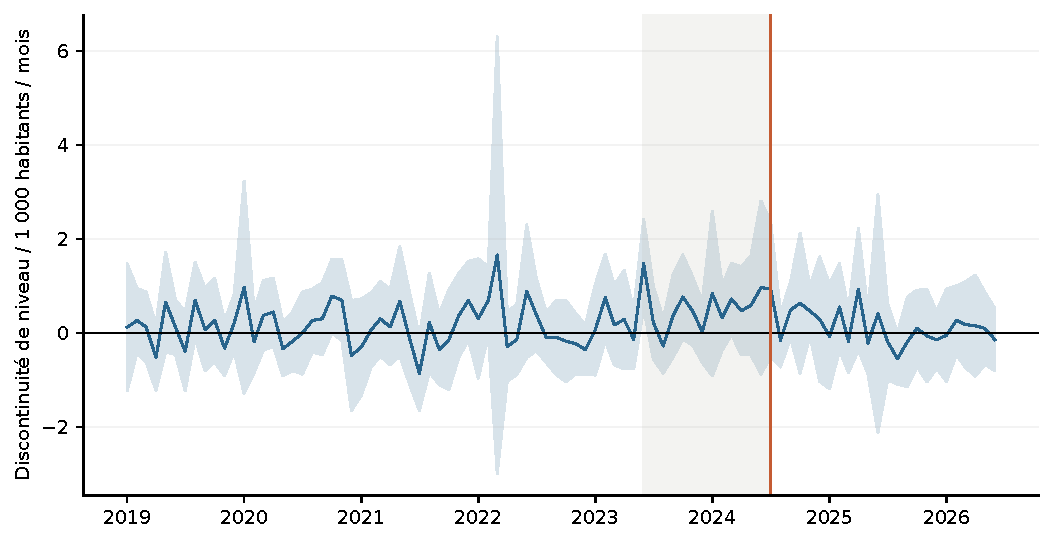
\includegraphics[width=\linewidth]{../results/figures/bassin_rd_monthly.pdf}\caption{Discontinuités de niveau au seuil de revenu des bassins}\label{fig:bassinRD}\notes{Côté de revenu faible moins côté de revenu élevé ; rayon fixe de 1\,000 euros, correction de biais et intervalles ponctuels HC3. Ces niveaux ne sont pas normalisés à un mois de référence. Zone grise : annonce–juin 2024. Les mois 2025–2026 sont descriptifs et ne relèvent pas tous du régime initial.}\end{figure}

Pour juillet–décembre 2024, le contraste corrigé est \BVRDCoef{} avec intervalle RBC–HC3 [\BVRDLo{} ; \BVRDHi{}]. Les quatre rayons montrent la sensibilité du lissage (tableau~\ref{tab:bassinRD}). Les composantes des communes retenues sont au nombre de \BVRDGroupN{} ; celles de l’ensemble des membres ne sont que \BVRDFullGroupN{}, avec \BVRDFullMaxShare{} \% des bassins dans la plus grande. Les erreurs types groupées sont ici plus petites, mais une structure aussi concentrée ne permet pas de les retenir comme une garantie de précision. Tous les calculs sont conservés dans l’annexe. Cette stratégie d’identification n’est pas retenue en raison de la continuité non établie et de la fragilité de l’inférence, indépendamment de la significativité du résultat après réforme.

\begin{table}[htbp]\centering\small\caption{Discontinuités administratives au seuil de bassin : tous les rayons fixés}\label{tab:bassinRD}\begin{tabularx}{\linewidth}{rrrrrX}
\toprule
Rayon (€) & BV ≤ seuil & BV > seuil & Linéaire & Corrigé & IC RBC, HC3 \\
\midrule
500 & 60 & 41 & 0,413 & 0,153 & [-0,465 ; 0,772] \\
750 & 96 & 62 & 0,336 & 0,466 & [-0,030 ; 0,962] \\
1000 & 119 & 79 & 0,255 & 0,444 & [-0,024 ; 0,912] \\
1500 & 169 & 100 & 0,330 & 0,202 & [-0,163 ; 0,567] \\
\bottomrule
\end{tabularx}
\notes{Immatriculations mensuelles par mille habitants de 2020, juillet–décembre 2024. Chaque rayon sert aussi à la correction de biais. BV : bassin de vie ; IC : intervalle de confiance. « Corrigé » désigne la correction statistique du biais de lissage, pas une correction de la sélection institutionnelle. Les intervalles HC3 supposent les bassins indépendants ; la dépendance et les diagnostics empêchent une interprétation causale.}\end{table}
\FloatBarrier

\subsection{Comparaisons larges, appariées et frontalières}
Le tableau~\ref{tab:main} montre des résultats différents selon les territoires comparés. Les contrastes larges et appariés sont proches de zéro, avec des intervalles couvrant des valeurs positives et négatives. Le contraste frontalier est positif. L’écart entre les trois comparaisons ne constitue pas, à lui seul, une preuve de déplacement spatial : les communes incluses et les conditions de comparaison diffèrent.
\begin{table}[htbp]\centering\small\caption{Contrastes juillet–décembre 2024 par rapport aux mêmes mois de 2019–2022}\label{tab:main}\begin{tabularx}{\linewidth}{Xrrrr}
\toprule
Comparaison & Contraste & Écart type & IC à 95 \% & p \\
\midrule
Large & -0,007 & 0,030 & [-0,065 ; 0,052] & 0,821 \\
Appariée dans le département & -0,017 & 0,042 & [-0,100 ; 0,066] & 0,682 \\
Frontières adjacentes & 0,146 & 0,048 & [0,051 ; 0,241] & 0,003 \\
\bottomrule
\end{tabularx}
\notes{Immatriculations mensuelles par mille habitants. Groupement EPCI pour l’échantillon large ; composantes EPCI–département pour les paires appariées ; composantes EPCI pour les frontières. Ces estimations ne sont pas validées comme effets causaux.}\end{table}

Dans l’échantillon frontalier, les créations d’unités légales localisables et la transformation $\log(1+n)$, où $n$ est le dénombrement mensuel brut d’immatriculations, présentent également des contrastes positifs. L’indicateur employeur est moins précis et son intervalle couvre zéro. Le contraste excluant les continuités enregistrées reste positif. Cette restriction réduit une catégorie particulière de changement administratif sans garantir que toutes les autres observations soient des créations économiques nouvelles.
\begin{table}[htbp]\centering\small\caption{Comparaisons frontalières selon l’indicateur observé}\label{tab:border}\begin{tabularx}{\linewidth}{Xrrr}
\toprule
Variable (échelle) & Contraste & Écart type & IC à 95 \% \\
\midrule
Immatriculations d’établissements / 1 000 & 0,146 & 0,048 & [0,051 ; 0,241] \\
Créations d’unités légales localisables / 1 000 & 0,105 & 0,037 & [0,032 ; 0,178] \\
Immatriculations d’établissements — log(1+nombre) & 0,023 & 0,009 & [0,005 ; 0,042] \\
Établissements employeurs actifs à la création / 1 000 & 0,020 & 0,011 & [-0,002 ; 0,041] \\
Sans continuité économique enregistrée / 1 000 & 0,130 & 0,039 & [0,053 ; 0,208] \\
\bottomrule
\end{tabularx}
\notes{\BorderPairs{} paires ; \EPCIComponentsN{} composantes EPCI. Les unités légales sont seulement celles dont le siège historique est localisable. L’emploi est un caractère administratif à la création, pas un effectif ou un emploi créé.}\end{table}

\subsection{Tendances préalables : un obstacle à l’interprétation causale}
Les courbes de niveau et les études dynamiques sont présentées aux figures~\ref{fig:trends}–\ref{fig:borderES}. Le test conjoint de 52 restrictions mensuelles sur janvier 2019–avril 2023, avec mai 2023 en référence, rejette les restrictions de trajectoire commune du modèle dynamique frontalier ($p<0{,}001$). Le test sur une fenêtre plus courte, juin 2021–avril 2023, ne rejette pas ($p=\ShortPreP$). Retenir uniquement ce dernier résultat aurait caché les différences préalables sur la période complète. Ces restrictions mensuelles sont plus fortes que la seule restriction de moyenne entre seconds semestres ; leur rejet affaiblit la justification du contrefactuel sans constituer un test direct de l’absence d’un effet FRR.

Le diagnostic retirant la saisonnalité propre à chaque paire rejette lui aussi les restrictions préalables ($p<0{,}001$ ; rang 41). Les trois contrastes annuels des seconds semestres 2019–2021 relativement à 2022 ne rejettent pas ($p=\AnnualPreP$), mais ce test de dimension plus faible impose une restriction plus faible et dispose d’une puissance différente. Il n’efface pas les différences mensuelles. Les comparaisons larges et appariées rejettent également les restrictions dynamiques complètes. Le très grand nombre de restrictions relativement aux groupes de l’échantillon apparié rend sa référence asymptotique fragile ; le diagnostic graphique et le résultat frontalier ne reposent pas sur cette seule valeur $p$.

\begin{figure}[htbp]\centering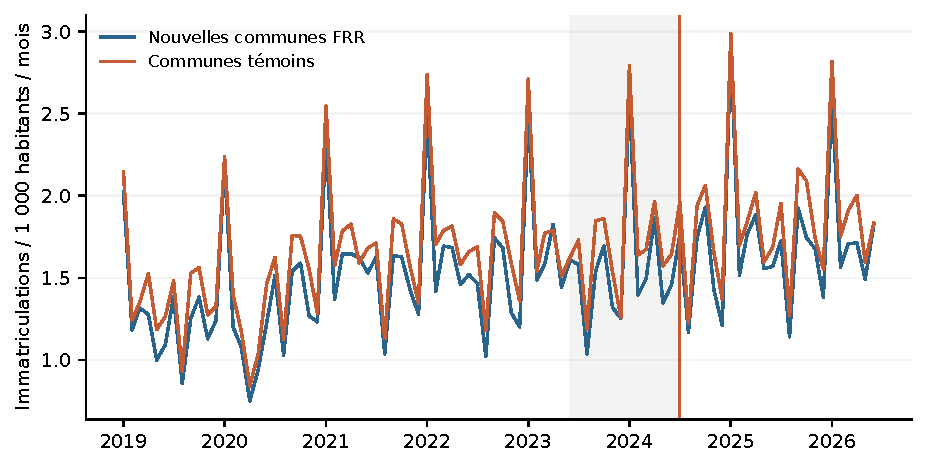
\includegraphics[width=\linewidth]{../results/figures/broad_trends.pdf}\caption{Évolution mensuelle des immatriculations : échantillon large}\label{fig:trends}\notes{Moyennes communales non pondérées. La zone grise va de l’annonce de juin 2023 à juin 2024 ; la ligne indique juillet 2024. Les observations de 2025–2026 fournissent un contexte descriptif, avec des régimes pouvant évoluer.}\end{figure}
\begin{figure}[htbp]\centering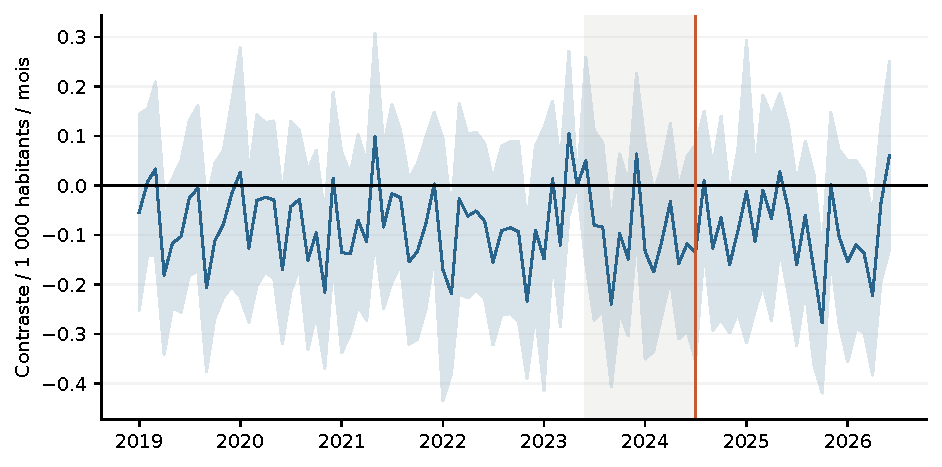
\includegraphics[width=\linewidth]{../results/figures/broad_event_study.pdf}\caption{Comparaison dynamique dans l’échantillon large}\label{fig:broadES}\notes{Mai 2023 en référence ; intervalles ponctuels à 95 \%, groupement EPCI. L’absence de significativité du contraste moyen ne prouve pas une absence d’effet causal national.}\end{figure}
\begin{figure}[htbp]\centering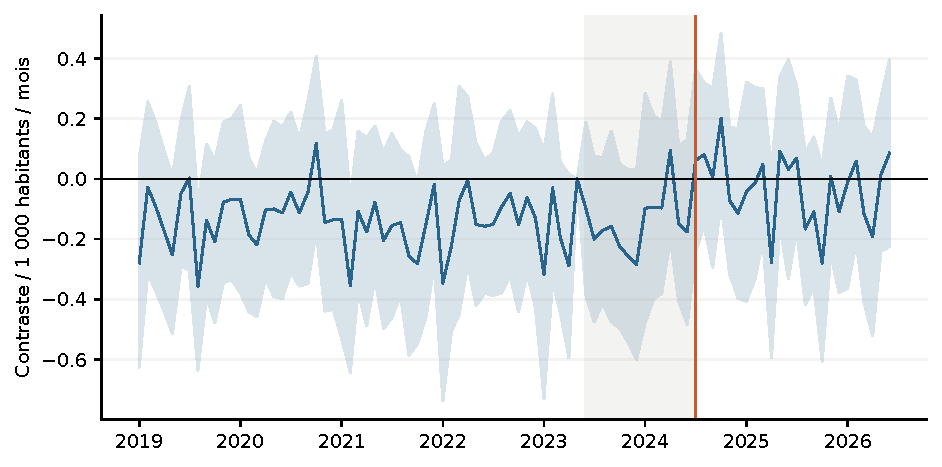
\includegraphics[width=\linewidth]{../results/figures/border_event_study.pdf}\caption{Comparaison dynamique dans les paires frontalières}\label{fig:borderES}\notes{Mai 2023 en référence ; effets fixes commune et paire–année-mois ; intervalles ponctuels à 95 \%, composantes EPCI. Les restrictions préalables complètes sont rejetées.}\end{figure}
\FloatBarrier

\subsection{Secteurs, modèles et robustesse numérique}
Les sept groupes sectoriels sont rapportés au tableau~\ref{tab:sectors} et à la figure~\ref{fig:sectors}. Aucun ne reste significatif au seuil de 5 \% après correction de Holm. Le contraste brut dans l’industrie manufacturière ne justifie donc pas une conclusion sectorielle choisie parmi les tests. Les données ne permettent pas de remplacer ces groupes par une mesure exacte du droit fiscal de chaque entreprise.
\begin{table}[htbp]\centering\small\caption{Exposition sectorielle : ensemble des groupes prédéfinis}\label{tab:sectors}\begin{tabularx}{\linewidth}{Xrrrr}
\toprule
Secteur & Contraste & Écart type & p brut & p Holm \\
\midrule
Commerce & 0,023 & 0,013 & 0,083 & 0,499 \\
Hébergement-restauration & 0,002 & 0,008 & 0,825 & 1,000 \\
Construction & 0,013 & 0,015 & 0,393 & 1,000 \\
Industrie manufacturière & 0,025 & 0,011 & 0,031 & 0,217 \\
Services professionnels & 0,008 & 0,012 & 0,516 & 1,000 \\
Santé humaine & 0,003 & 0,008 & 0,674 & 1,000 \\
Services de proximité & -0,003 & 0,012 & 0,825 & 1,000 \\
\bottomrule
\end{tabularx}
\notes{Paires frontalières ; par mille habitants et par mois ; correction de Holm au sein de la famille des sept tests.}\end{table}
\begin{figure}[htbp]\centering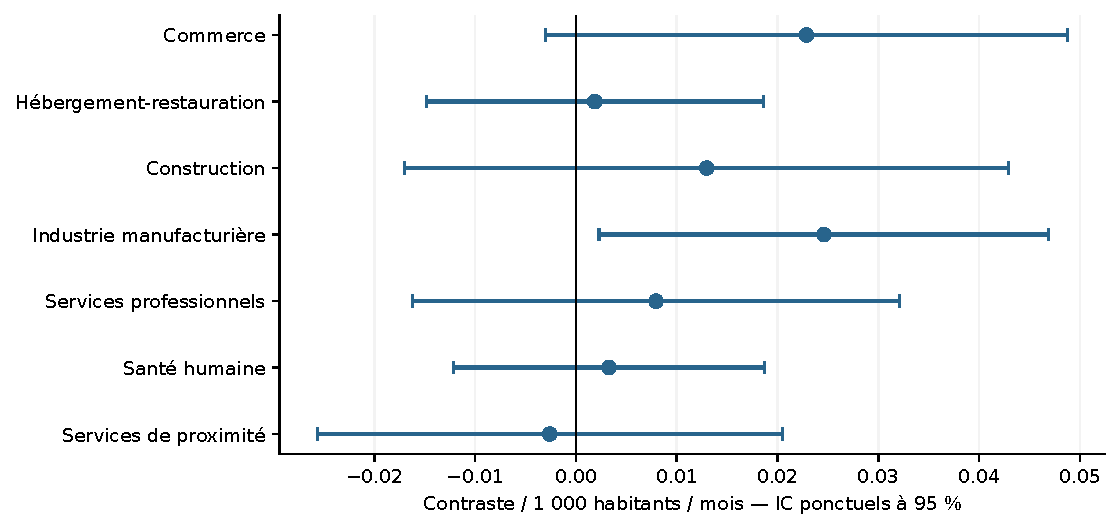
\includegraphics[width=\linewidth]{../results/figures/sector_heterogeneity.pdf}\caption{Contrastes sectoriels frontaliers et incertitude}\label{fig:sectors}\notes{Les intervalles sont ponctuels, sans correction familiale ; les conclusions tenant compte des tests multiples sont celles du tableau~\ref{tab:sectors}.}\end{figure}

Le modèle conditionnel de Poisson donne un rapport de taux de \PPMLRatio{}, sur \PPMLPairs{} paires informatives ; \PPMLExcluded{} paires sont exclues. Les principales variantes de fenêtre, de population et d’échantillon conservent un contraste frontalier positif. Les fausses dates de juillet 2021 et de juillet 2022 ne donnent pas de contraste significatif. Juillet 2023, après l’annonce, présente un contraste négatif proche du seuil usuel et ne constitue pas un placebo sans politique. Les résultats numériques et leur stabilité sont distincts de la crédibilité de la tendance contrefactuelle.
\begin{table}[htbp]\centering\small\caption{Robustesse des contrastes frontaliers}\label{tab:robust}\begin{tabularx}{\linewidth}{Xrrrr}
\toprule
Spécification & Paires & Contraste & Écart type & p \\
\midrule
Fausse réforme : juillet 2021 & 774 & -0,067 & 0,042 & 0,111 \\
Fausse réforme : juillet 2022 & 774 & 0,017 & 0,048 & 0,720 \\
Seul second semestre 2022 en référence & 774 & 0,133 & 0,054 & 0,015 \\
Douze mois, hors futures FRR+ & 683 & 0,132 & 0,037 & $<0{,}001$ \\
Pondération par population de la paire & 774 & 0,086 & 0,040 & 0,036 \\
Frontières dans le même département & 717 & 0,144 & 0,050 & 0,005 \\
Deux communes sous 25 000 habitants & 772 & 0,147 & 0,048 & 0,003 \\
Seul second semestre 2019 en référence & 774 & 0,168 & 0,057 & 0,004 \\
Juillet 2023 : période d’annonce & 774 & -0,097 & 0,049 & 0,051 \\
\bottomrule
\end{tabularx}
\notes{Même mesure principale et composantes EPCI. La fenêtre de douze mois exclut les communes devenant FRR+, mais ne supprime pas toutes les autres évolutions juridiques. Les variantes ne remédient pas au rejet des tendances préalables.}\end{table}

\section{Espace, emploi et maintien administratif}
Le tableau~\ref{tab:spatial} compare le nombre d’immatriculations de chaque côté et leur somme. Les immatriculations augmentent à la fois dans les communes FRR et chez leurs témoins voisins. Il n’existe donc pas, dans ces moyennes, un schéma simple de hausse du côté traité accompagnée d’une baisse du côté témoin. La somme augmente aussi. Toutefois, une variation temporelle brute de cette somme ne fournit pas son contrefactuel. Le modèle linéaire à effets fixes paire–année-mois retire la composante commune des taux par habitant ; il n’identifie pas l’effet sur la somme des dénombrements. Le modèle de Poisson conditionne sur cette somme sans en estimer l’évolution contrefactuelle. Aucune conclusion de création nationale nette ne peut en être tirée.
\begin{table}[htbp]\centering\small\caption{Entrées de part et d’autre des frontières : description en nombres d’immatriculations}\label{tab:spatial}\begin{tabularx}{\linewidth}{Xrrr}
\toprule
Série & Pré / mois / paire & Après / mois / paire & Variation \\
\midrule
Côté FRR & 1,503 & 1,718 & 0,216 \\
Côté témoin voisin & 1,816 & 2,002 & 0,186 \\
Somme des deux côtés & 3,319 & 3,720 & 0,402 \\
\bottomrule
\end{tabularx}
\notes{Moyenne mensuelle par paire. Référence : seconds semestres 2019–2022 ; après : second semestre 2024. Les variations sont descriptives, sans contrefactuel extérieur des totaux régionaux.}\end{table}

Une réponse indirecte positive ou négative du témoin reste possible même si son niveau total augmente. Inversement, la différence entre comparaison frontalière positive et comparaison large proche de zéro peut résulter d’une hétérogénéité des territoires ou de tendances différentes. Ni cette divergence ni le tableau des sommes ne permettent d’isoler une relocalisation. Un échantillon extérieur à la zone d’influence, avec des tendances comparables et une définition préalable de cette zone, serait nécessaire pour poursuivre cette question.

L’indicateur d’employeur ne donne pas de preuve robuste d’une hausse des immatriculations d’établissements employeurs. Il ne mesure ni le nombre de travailleurs, ni l’emploi total local. Les tranches courantes d’effectifs ne sont pas utilisées pour fabriquer un résultat sur l’emploi historique. Les comparaisons supplémentaires de catégories juridiques et de transitions administratives sont présentées dans l’annexe.

Les taux de maintien à douze et dix-huit mois sont également descriptifs. La politique pourrait modifier le type d’établissement qui entre ; comparer uniquement les entrants après la réforme revient alors à conditionner la comparaison sur un résultat du traitement. Les écarts de taux entre cohortes ne sont donc pas des effets individuels sur la survie. Les états inconnus sont séparés et des bornes extrêmes les traitant tous comme actifs ou fermés sont conservées dans les données de réplication.

L’hétérogénéité par densité descriptive, ajoutée après les résultats, est exploratoire. Elle n’est pas une preuve d’interaction causale. Les niveaux légaux de revenu et de densité sont maintenant reconstruits pour vérifier l’assignation ; ils ne valident pas rétrospectivement cette hétérogénéité. Aucune concentration d’effets causaux dans les territoires pauvres ou en déclin démographique n’est établie.

\section{Discussion et limites}
Le contraste frontalier positif décrit une modification relative d’immatriculations dans un sous-échantillon de voisins. Pour lui donner une interprétation causale, il faudrait justifier une trajectoire contrefactuelle qui ne soit pas contredite par les différences préalables et distinguer les effets indirects subis par les témoins. La correction de saisonnalité ne supprime pas le premier problème. Une extrapolation de tendance linéaire conserve un contraste positif, mais ajoute une hypothèse de modèle ; elle n’est pas une validation indépendante.

L’épisode FRR se distingue des anciennes ZRR par sa transition juridique et ses nouveaux périmètres. Les résultats antérieurs de \citet{ref1} ne prouvent pas que cette réforme soit inefficace. De même, les constats urbains de déplacement \citep{ref2,ref4} ne prouvent pas que la hausse relative observée ici soit une relocalisation. Ils définissent les questions que les résultats actuels ne permettent pas de trancher. La différence entre attraction locale, nouvelles activités et bénéfice pour les résidents demeure centrale.

L’exposition observée est une désignation territoriale. Le recours effectif aux exonérations, les décisions locales de CFE et de TFPB et le respect des conditions fiscales ne sont pas mesurés. Une courte fenêtre peut manquer des réponses différées, notamment pour les avantages locaux applicables aux créations ou rattachements de 2024 à partir des impositions de 2025. Cette difficulté interdit de convertir un contraste proche de zéro en jugement définitif sur le dispositif. Elle ne justifie pas non plus de prolonger sans distinction la fenêtre principale dans un régime renforcé rétroactif.

La reconstruction ouverte apporte une traçabilité : textes originaux, codes historiques, maintien des effets ZRR, calendrier et géographie sont séparés. Le contrôle des dates historiques évite de classer une entreprise selon son état ou son siège actuel. La qualité de ces transformations ne garantit cependant pas la validité économétrique. Le contrôle sur vingt cellules a vérifié des calculs et des correspondances ; ce n’est pas une preuve de complétude générale ni de causalité.

Une évaluation ultérieure devrait préciser les voies de classement effectivement retenues, obtenir un contrefactuel avec une trajectoire crédible, et définir une stratégie pour les effets spatiaux. Une analyse de sensibilité des tendances doit afficher les restrictions sur les écarts futurs au lieu de sélectionner un test préalable favorable. Un suivi supplémentaire enrichirait les résultats économiques seulement si les indicateurs et les modifications de régime sont traités séparément. Aucune recette d’extrapolation n’est présentée ici comme réparation automatique.

\section{Conclusion}
Les données publiques permettent de reconstruire les nouvelles communes FRR, de distinguer les établissements des unités légales et d’examiner les premières évolutions mensuelles des immatriculations. Les comparaisons larges et appariées sont proches de zéro ; les comparaisons entre communes adjacentes présentent un contraste positif. Les diagnostics complets de tendances préalables ne permettent toutefois pas de valider ces comparaisons comme une évaluation causale de la réforme. Aucun résultat n’établit un gain national net, une hausse de l’emploi ou un effet causal sur la survie.

La reconstruction retrouve les indicateurs de 2020 et leurs périmètres, sépare les voies obligatoires de leurs possibilités supplémentaires, et confronte leur union à l’ensemble de la liste métropolitaine initiale. Elle montre aussi que les nouveaux bénéficiaires disponibles autour des seuls seuils EPCI sont très peu nombreux. L’analyse au seuil des bassins porte sur davantage d’unités comparables, mais présente des différences substantielles de couverture et de trajectoires préalables, ainsi qu’une dépendance géographique concentrée. Ces constats précisent les conditions d’une évaluation future, sans imposer de conclusion positive ou négative sur la politique. Les données de traitement, les indicateurs administratifs et les diagnostics constituent les résultats reproductibles de ce travail.

\section*{Données, code et intégrité}
Toutes les données proviennent de sources officielles gratuites. Le dossier de réplication contient scripts, liens et empreintes de sources, dictionnaires, agrégats, tables, figures et rapports de vérification. Les fichiers bruts SIRENE et les intermédiaires individuels ne sont pas redistribués. Les conditions de chaque source restent applicables ; la licence du manuscrit ne remplace pas celles des bases utilisées. Les données géographiques et leurs dérivés sont identifiés séparément dans la notice de réutilisation. Les contributions originales du manuscrit et de l’annexe sont mises à disposition sous \source{https://creativecommons.org/licenses/by/4.0/}{CC BY 4.0}, avec maintien des droits et attributions des sources tierces. Le code original est sous licence MIT. Le fond \source{https://www.data.gouv.fr/datasets/contours-administratifs}{Contours administratifs} et ses bases dérivées conservent les conditions ODbL 1.0 ; les méthodes complètes de reconstruction sont fournies.

\section*{Déclaration relative à l’utilisation d’outils d’intelligence artificielle}
Codex (OpenAI) a contribué de manière substantielle à la recherche documentaire et institutionnelle, aux scripts de téléchargement et de nettoyage, aux programmes d’estimation, aux contrôles de données et de calculs, aux figures et tableaux ainsi qu’à la rédaction et à la révision linguistique en français. Des agents d’IA distincts ont réalisé des examens internes de l’institution, des estimateurs, des données et de la langue. Ces contrôles ne sont ni une expertise par des pairs humains ni une relecture par une personne dont le français est la langue maternelle. Aucun outil d’IA n’est auteur. Les choix méthodologiques, leur chronologie et les vérifications effectivement réalisées sont documentés dans le dossier de réplication. Kun Huang est le seul auteur humain ; la responsabilité du contenu, des interprétations et de la décision de diffusion lui appartient.

\bibliographystyle{plainnat}
\bibliography{references}
\end{document}
